\documentclass{sig-alternate-05-2015}

\usepackage{underscore,amsmath,amssymb,graphicx}
\usepackage{algorithm}% http://ctan.org/pkg/algorithms
\usepackage{algpseudocode}% http://ctan.org/pkg/algorithmicx
\usepackage{url}

\DeclareRobustCommand{\ttfamily}{\fontencoding{T1}\fontfamily{lmtt}\selectfont}

\hyphenation{light-weight}

\begin{document}

% Copyright
\setcopyright{acmcopyright}

% DOI
\doi{10.475/123_4}

% ISBN
\isbn{123-4567-24-567/08/06}

%Conference
\conferenceinfo{Euro MPI}{Aug XX--YY, 2016, XXX, YYY, ZZZ}

\title{Toward million communicating threads}

\numberofauthors{3}
\author{
\alignauthor
Hoang-Vu Dang\\
\affaddr{Department of Computer Science}\\
\affaddr{University of Illinois at Urbana-Champaign}\\
\email{hdang8@illinois.edu}
%
\alignauthor
Marc Snir\\
\affaddr{Department of Computer Science}\\
\affaddr{University of Illinois at Urbana-Champaign}\\
\email{snir@illinois.edu}
%
\alignauthor
William Gropp\\
\affaddr{Department of Computer Science}\\
\affaddr{University of Illinois at Urbana-Champaign}\\
\email{wgropp@illinois.edu}
}

\maketitle

\abstract{
  We present the design, implementation and analysis of an efficient runtime
  which supports of million concurrently communicating threads using Message
  Passing Interface.
}

\section{Introduction}
Message Passing Interface (MPI) has been implemented by several vendors. On
Blue Gene machine, MPICH \cite{mpich} is the de-factor implementation, likewise
on Infiniband machine, we have MVAPICH \cite{mvapich}. Cray has their own
customization on top of MPICH called CrayMPI; Intel similarly implements
IntelMPI. OpenMPI is another effort from Open-source collaboration of several
industry and academic vendors \cite{openMPI}.  Each vendor relies on 
their best knowledge of the underlying computing machine and network
architecture to optimize their implementation. For examples, the implementation
might reduce latency by accessing directly the low-level network-API or
optimize critical path using specialized instructions.

Recently, because of the increasing in the number of processor cores within a
computing board, there raises a need of running MPI efficiently in threaded
environments. Although MPI specification requires all of its procedures to be
thread-safe, MPI implementations are not originally designed to optimize for
using multiple threads: OpenMPI latest version still does not
provide a stable support of MPI\_THREAD\_MUTLIPLE \cite{openmpifr},  MPICH suports thread-safety
via a coarse-grain locking which essentially serialized all MPI code. The
research to replace coarse-grain locking is still undergoning \cite{mpilock}, but the
progress is slow because the existing software stack is only optimized for
single-core performance. For example, there are significant number of global
variables shared among various component of a MPICH. Global variables which
implements stack, queue or hash-table can be replaced with concurrent data
structure, others might be protected with finer-grains lock.  However, locks
and concurrent data structure has overhead could be added to  the critical path
and reduces performance of single-threaded applications.

On the other hand, communication in multiple threads is troublesome for many
reasons. Data movement between processors could cache trashing or false sharing
if taken care of. Processors can becomes under-ultilize because threads execute
I/O operations can be preempted. Resource management have to consider locality
and efficient concurrent accesses since they are shared among processors. Last
but not least, kernel thread context-switching is costly, increasingly with the
number of threads. Several studies have reported significant overhead for
performing MPI concurrently in many threads \cite{threadissue, mpilock}.

Because of the lack of efficient multi-threaded implementation, to our best
knowledge, there is no production application that uses the thread-safety
feature of MPI. What has been ended up is application running MPI in a ``Thread
Funnelled'' mode i.e. only one thread is allowed to execute MPI procedure;
other threads are used only for computation. This leads to a fairly restrictive
programming model, in which communication and computation code appears in
different phases or procedures. This approach often uses MPI non-blocking
features to allow overlapping between computation and communication and hope
the MPI runtime will be able to make communication progress behind the scene.
In practice, to support better asynchronous communication, user of MPI
implementations often need to enable a flag to request the runtime to spawn a
dedicated polling thread for progressing the communication (e.g.,
MPICH_ASYNC_PROGRESS flag in MPICH/MVAPICH).

The solution that we have seen for existing MPI implementation to adopt
multi-core machine is thus ad-hoc and inefficient. In this paper, we present an
approximate implementation of MPI point-to-point communication which takes into
account of multi-core machine by design. Our implementation is approximate
since we shall relax some semantics requirement of MPI. We argue that our
design and algorithms for this relaxation is able to achieve efficient
implementation, yet do not restrict applications from using MPI effectively.
More complex MPI semantics and functionality can be built on top of our
point-to-point communication. By using this bottom-up strategy, we provide an
insight on the minimal cost to implement MPI, accurately to the number of
memory accesses. We summarize our most signfinicant contributions as follows:
\begin{itemize}
  \item A light-weight thread scheduler using bit-vector which achieves
single-instruction for signalling continuation. 
  \item An constant time overhead algorithm for MPI point-to-point communication
utilising a specially designed concurrent wait-free hash-table.
  \item A resource-aware locality-aware concurrent memory pool for packet management.
  \item A MPI runtime design for scaling up to million communicating threads.
\end{itemize}

Our paper is organized as follows. The next section describes our runtime
architecture from the high-level design to individual components. We present
our implementation details and optimization in Section \ref{sec:impl}. Section
\ref{sec:exp} discusses experiment and results. Section \ref{sec:related} gives
an overview of some related works. Finally Section \ref{sec:conclusion} concludes
our study.


\section{Runtime Architecture}
\label{sec:runtime}
\subsection{High-Level System Design}
We first identify the complication of MPI code is on the message matching
mechanism. MPI point-to-point procedures (Send/Recv) facilitate matching
messages by tagging each with an integer in addition to destination and
communicator. The implementation uses several queues data structure to store
incoming requests and messages. For example, the unexpected queue store arrived
messages without a matching request; the posted queue will store the pending
requests without matching messages. Depending on different arrival order,
traversing, insertion or deletion of entries into queues will be issued. In a
concurrent setting, these are critical section that need to be protected. An
efficient lock-free control of these operations are non-existent even though
individual queue could be implemented efficiently.  Moreover, when the number
of concurrent communication increases, traversing a queue requires linear time
to the size of pending requests.

We propose an implementation MPI based on the following assumptions:
\begin{itemize}
  \item Large number of concurrent threads Threads are lightweight; they are
    scheduled by a user-space scheduler that understands synchronization
    objects.
  \item The implementation is optimized for the case where MPI_ANY_SOURCE and MPI_ANY_TAG are not used.
  \item No concurrent send and receive having the same signature, thus we do not yet worry about odering.
  \item The NIC can be accessed in user space; it has its own routing tables,
    in order to translate ranks in MPI\_COMM\_WORLD to physical node addresses;
    it has page tables, in order to translate virtual addresses to physical
    addresses.
  \item We consider only x86_64 machine, however the technique is general
    enough to port to other architecture which supports atomic exchange and
    atomic bit manimupation.
\end{itemize}

The key data structure for communication is a lock-free hash table which stores
both unsolicited incoming messages and outstanding receives. Since we assume
there are no don't cares, we can hash by source and tag. We focus on critical
operations, the creation of communicators or of datatypes is not (yet)
address. We also ignore, for the time being, one-sided operations.

The runtime is an integrated system of a user-level thread (ULT) scheduler and
a communication server. The ULT provides a low latency thread management while
the server is a kernel-thread dedicating to message delivery. The two
components interact using the afortmentioned hash-table.  Our primary goal is
to design an algorithm and optimize to minimize the latency of this
interaction. A failure to achieve this goal simply adds extranous overhead to
single threaded application and might not achieve significant benefit that
justifies its cost. We shall also show that our design allows optimization space
to be reduced to optimizing a few neccessary operations.

Resource management is another important issue. Aside from communication
context such as connections and NIC-provided control data which we maintains
per communication server, we have to maintain a pool of packets structure. The
pool is the second shared data structure of the runtime.  Each packet is used
for storing control and message data to deliver to network device.

\begin{figure*}
  \centering
  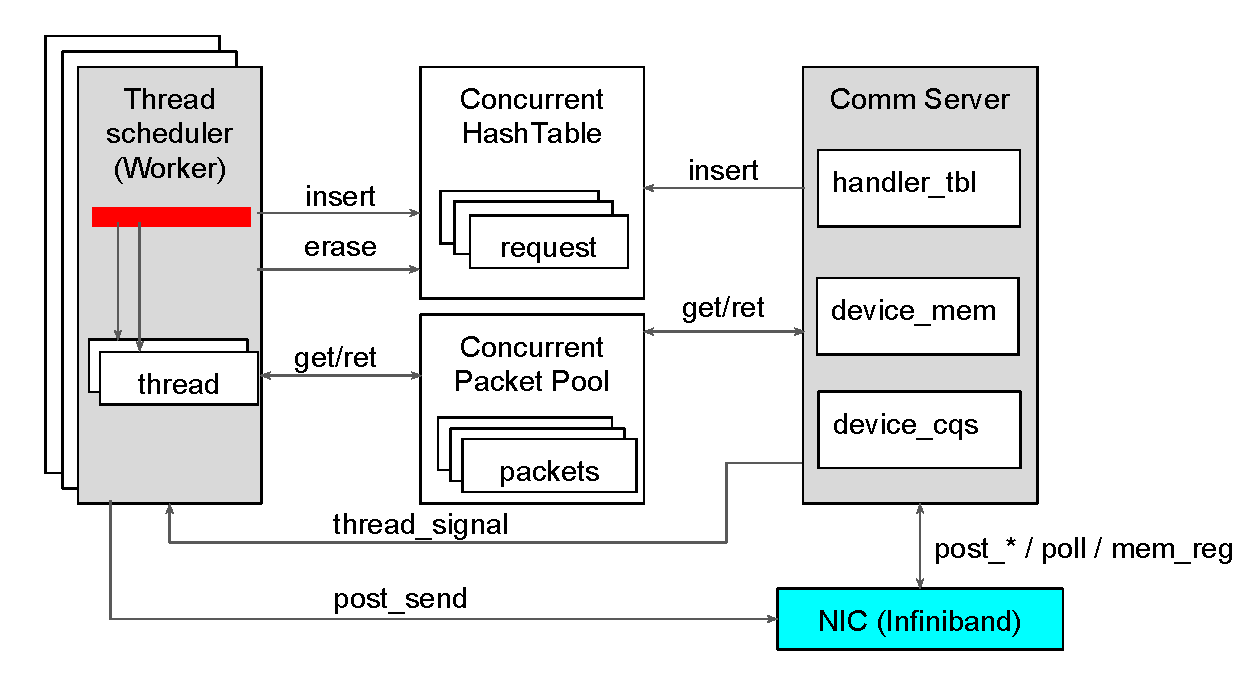
\includegraphics[width=.6\textwidth]{fig/runtime.pdf}
  \caption{MPI Runtime Architecture for multi-threaded executions}\label{fig:overall}
\end{figure*}

Figure \ref{fig:overall} shows the overall architecture of our described
runtime system.

\subsection{Point-to-Point Message Passing Algorithms}
We now describe an algorithm and its data structure that facilites the
point-to-point communication in Message Passing semantics. Our algorithm relies
on a specialized concurrent hash-table $H$ defined as follows.

We denote a tuple $(k,v) \in H$ when $v$ is stored in the hash-table using the
key $k$. At initialization, for any key $k$, only the tuple $(k,\bot)$ are
stored in the table. The hash-table has two operations: 

\begin{itemize}
  \item $H.\text{insert}(k,v)$: attempt to replace value of key $k$ by $v$.
  \item $H.\text{empty}(k)$: replace value of key $k$ by $\bot$
\end{itemize}

Additionally, let $H_t$ denote a state of $H$ which is a set of all key-value
pair stored in $H$ at time $t$, $H_{t_0}$ denote the state of $H$ before a
operation and $H_{t_1}$ denotes the state of $H$ after a operation;
$\mathbb{K}, \mathbb{V}$ denote the key and entry space. In a sequential
history, we have the following legal semantics:

\begin{equation}
  \text{insert}(k, v) = \left\{
    \begin{array}{@{}l@{\thinspace}l}
      v \iff (k,\bot) \in H_{t_0}, (k,v) \in H_{t_1}\\
      v' \iff (k,v') \in H_{t_0}, (k,v') \in H_{t_1}
    \end{array}
    \right.
\end{equation}
\begin{equation}
  \text{empty}(k) = \text{success} \iff  (k,v) \in H_{t_0}, (k,\bot) \in H_{t_1}
\end{equation}
\begin{equation}
  \forall k_0 \in \mathbb{K}, \nexists {(v_0, v_1) \in \mathbb{V}}
  \mid {{v_0 \ne v_1} \wedge {(k_0, v_0), (k_0, v_1)} \subset H_{t}}
\end{equation}

That is, (1) means that \texttt{insert} succeeds only if the entry being stored
with $k$ at the time of insertion is $\bot$.  In that case, $(k,\bot)$ is
replaced with $(k, v)$. Otherwise, the operations fail and existing value is
returned i.e. no changed are made to $H$. In contrast, \texttt{erase} as in (2)
is always successful, which replaces any value $v$ with the input $k$ with
$\bot$, essentially removing $v$ from the hash-table. The (3) equation is the
consistency requirement for hash-table, which means for each key we allow
only one value associated with it.

In a concurrent setting, we further require the hash-table to be
\textit{linearizable}.  This means we ensure firstly safety and correctness
property. Secondly, we ensure operations take affect in a real-time order.
This is a strong guarantee however is neccessary to implement MPI semantics
which have operations executed in program order. Lastly, linearizability is
\textit{composable} which allows us to correctly use the hash-table to
implement other concurrent objects.

Message delivery in general can be implemented in two way: \textit{eager} or \textit{rendevouz}
protocol. Eager protocol is used when the target buffer is not known to the
sender. Thus, an copy is made into an intermediate buffer - usually packed with
other control data to deliver to the network. This also allows the Send
operation to return immediately as the buffer can be reused.  This protocol
however becomes inefficient when message size gets larger, typically larger
than the L2 or L3 cache size i.e. the cost of data movement is significant.
When this is the case, we switch to rendevouz protocol in which the data is
delivered directly from the source buffer to the target buffer by the NIC thus
saving extra copies.  The protocol however requires some control messages to
exchange control data and signal completion.

\subsubsection{Eager protocol}

\begin{algorithm}
  \caption{Eager-message send/recv for thread}
  \label{algo:short}
  \begin{algorithmic}[1] % The number tells where the line numbering should start
    \Procedure{Send-Eager}{$b, s, d$} \Comment: buffer, size, destination signature 
      \State $p$ = pkpool.get()
      \State Set packet header $p.d$ to $d$
      \State Copy $b$ to $p.b$
      \State Post $p$ to network for send.
    \EndProcedure
    \\
    \Procedure{Recv-Eager}{$b, s, d$} \Comment: buffer, size, source signature 
      \State Create a request $r$ = $(b,s,d, (\omega, \Gamma))$
      \State Create hash-value $v$ from $r$.
      \State Create hash-key $k$ from $d$.
      \State $v' = H.\text{insert}(k,v)$
      \If {$v' \ne v$}
        \Comment: insertion fail
        \State Copy $v'.p.b$ to $b$
        \Comment: message arrived, copy data.
        \State pkpool.ret($p$)
      \Else
        \Comment: insertion success
        \State \texttt{ThreadWait}()
        \Comment: message not arrived, wait.
      \EndIf
      \State $H.\text{erase}(k)$
    \EndProcedure
  \end{algorithmic}
\end{algorithm}

\begin{algorithm}
  \caption{Eager-message packet handler for communication server}
  \label{algo:server-short}
  \begin{algorithmic}[1]
    \Procedure{Recv-Eager-Packet}{p}
      \State Create hash-value $v$ from $p$.
      \State Create hash-key $k$ from $p.d$.
      \State $v' = H.\text{insert}(k,v)$
      \If {$v' \ne v$}
        \Comment: insertion fail.
        \State Copy $p.b$ to $v'.r.b$
        \Comment: thread arrived, copy data.
        \State \texttt{ThreadSignal}($r.\Gamma$)
        \State pkpool.ret($p$)
      \Else
        \Comment: insertion success.
        \State \Return
        \Comment: thread not arrive, nothing to do.
      \EndIf
    \EndProcedure
  \end{algorithmic}
\end{algorithm}

The pseudocode for eager protocol is listed in Algorithm \ref{algo:short} and
\ref{algo:server-short} for worker thread and communication server
respectively. The basic idea here is that the thread and the communication
server could use the results from hash-table insertion to coordinate the
matching of messages and request. 

If the communication server succeeds with the hash insertion, the server knows
the receiving request has not been posted and it returns immediately. A thread
later comes, eventually fails the insertion but finds a packet with the needed
data to work with. On the other hand, if the thread is the one who succeeds,
the request is then inserted into the hash-table with the synchronization
object.  The thread is yielded by executing \texttt{ThreadWait}. The worker is
now free to do other works. When the associated packet arrived, the server will
fail the insertion and find the request with the attached synchronization
object. It now can mark the thread as schedulable using \texttt{ThreadSignal}
so when the worker is available it will pick up the works with the available
data.

Since there is no need for linear searching, our matching algorithm achieves a
constant time complexity as long as operation of thread scheduler, pool and
hash-table is also constant time.

\subsubsection{Rendevouz protocol}
A rendevouz protocol have the same algorithm as short protocol after we have
exchanged the control message via eager-protocol. The control messages 
includes two messages: a RTS (ready-to-send) issued by the sender, a RTR
(ready-to-receive) issued by the receiver. By then, the sender and the receiver
has known the addresses of each other buffer and they can perform
communication.  The data transfer could be optimized further using the
Remote Direct Memory Access (RDMA) feature of modern Network Interface
Controller (NIC).  Several researchs has focused on optimizing this operation.

As an effect of our assumption, in this protocol we can save one control
message i.e. the RTS.  The reason is we do not have wild-card, the sender and
receiver knows exactly their target.  We only require the receiver to send its
buffer to the sender. The sender can follow up by issuing an RDMA.  Analogous
to the eager protocol, whenever the sender or receiver is required to wait for
a matching message it will perform \texttt{ThreadWait}, and later when the
message has arrived the communication server will perform a
\texttt{ThreadSignal}.

Specifically, the sender waits when the RTR message has not arrived or when
RDMA is pending. In both situation the server wake up the sender thread when
RDMA has completed. The receiver after issuing the RTR will wait until the
signal that RDMA has finished arrived and data is now available.

\subsection{Critical Operations Discussion}
Clearly, optimizing the hash-table, the packet pool and the thread scheduler
operations are the key to achieve good performance for our protocols. One could
achieve $O(1)$ amortized in complexity however, an efficient implementation
requires optimizing for the constant factor. Ideally, we want these operations
to be \textit{wait-free} to ensure progress and minimizing the number of memory
accesses and possible cache misses. In the next section, we describe the
implementaion of each of the three components and show how we could optimize
toward our goals.


\section{Runtime Implementation and Optimization}
\label{sec:impl}
\subsection{Thread scheduler}
As mentioned earlier, our scheduler implements User-Level Thread (UTL). The
user specifies the number of workers which are implemented with POSIX thread
and pinned to a specific core. The context-switching mechanism is similar to
that of Argobots and Boost coroutines, we make use of \texttt{fcontext}. The
idea is to maintains a separate stack for each thread. A few registers
(including the program counter) is saved and restored from an allocated space
in the stack. Morever, the context-switching is designed to not involve
Operating System (OS) system call, thus by-passing kernel code. This overall
reduces the latency of switching to a new context to less than a hundred
cycles.

Rather than designing a general purpose ULT, we focus on the two most important
operations for synchronization purpose: \texttt{ThreadWait} and
\texttt{ThreadSignal}. A possible implementation is \textit{condition
variable}. This is the typical mechanism in POSIX thread, and other ULT
library.  Condition variable is a generic container which can
be used as a building block for many other synchronization primitives. However,
it is still expensive as in general it requires a mutex lock and some queue
traversal when many threads are blocking.  An alternative is to use a
busy-waiting synchronization flag which has lower latency. However this is
considered even worst for scaling since the processor spends useless time
polling. Qthreads implements a slight modification notion of condition variable
namely \textit{full-empty bit}. However, internally each object is a waiting
queue and rescheduling requires expensive traveral of this queue to find
runnable threads and insert back to run queues.

Our thread scheduler targets a constant time overhead for both afortmentioned
operation. Marking a thread as runnable or waiting is only a single x86
instruction. The idea behind our thread scheduler is a novel use of bit-vector.
Rather than using a queue to implement a set of runnable thread, each bit in
the bit-vector indicates a schedulable thread. When a worker is created, it is
given a unique worker id, denotes as $\omega$.  When a thread is created by a
worker, it is assigned an unique id $\Gamma$ within the range of $[0,M-1]$, for
$M$ is the maximum concurrent threads for that worker.  For example, using a
vector of $8$ 64-bit words, we allow up to $512$ concurrent threads per worker.
A pair $(\omega, \Gamma)$ uniquely defines a thread in the system at a point in
time. During thread's creation time, the associated $\Gamma$ bit in its
bitvector structure is marked so that when the worker is free it will attempt
to schedule that thread to run. Algorithms \ref{algo:thread} further describes
our scheduling algorithms. 

\begin{algorithm}
  \caption{Thread scheduler}
  \label{algo:thread}
  \begin{algorithmic}[1]
    \Procedure{Scheduling}{$\omega$, V} \Comment{worker, bit-vector}
    \While {!$\omega$.stop} \Comment{loop until user ask to stop}
      \For{word in V}
      \If{word $\ne$ 0}
        \State localWord = 0
        \State AtomicExchg(word, localWord)
        \While {localWord64 $> 0$}
          \State b = FindFirstSet(localWord)
          \State localWord = FlipBit(localWord, b)
          \State ContextSwitch($b$)
        \EndWhile
      \EndIf
      \EndFor
    \EndWhile
    \EndProcedure
  \end{algorithmic}
\end{algorithm}

\begin{algorithm}
  \caption{Thread Operations}
  \label{algo:thread-ops}
  \begin{algorithmic}[1]
    \Procedure{ThreadWait}{}
      \State ContextSwitch($\omega$)
    \EndProcedure
    \\ 
    \Procedure{ThreadSignal}{sync}
      \State AtomicBitSet(sync.$\omega$.V, sync.$\Gamma$)
    \EndProcedure
  \end{algorithmic}
\end{algorithm}

The scheduler works at 64-threads granularity instead of 1-thread traditionally.
By using an atomic exchange instruction to swap the interested word to local variable, we
are able to continously perform read/write from/to this variable without
accessing the main memory. This is not only ensures progress property for all
threads because we can schedule them in order, it solves the problem of having
no atomic read-modify-write instructions operating at bit level.

Algorithms \ref{algo:thread-ops} describes the two thread operations.
\texttt{ThreadWait} simply switch back to the worker scheduler based on current
worker id (i.e. $\omega$) On the other hand, \texttt{ThreadSignal} shall access
the bit-vector and atomically set the bit in the appropriate word based on the
the same information stored in the synchronization object. $\omega$ and
$\Gamma$ are stored in thread local-storage of the worker, and is updated
whenever a new context is switch to.

There are couple of issues worth discussing on the above design.  Firstly, note
that \texttt{ThreadWait} is executed in the same kernel thread as the thread
scheduler associating with the running ULT while \texttt{ThreadSignal} can be
executed anywhere. Thus, It is errornous to perform \texttt{ThreadSignal}
multiple times on the same object since they will be treated as one or more
signal depending on the time the worker looks at the bit-vector. It is also
erronous to \texttt{ThreadWait} when the associted \texttt{ThreadSignal} has
been performed. In practise for each MPI request we use an additional flag to
indicate whether the signal has been executed before performing the
\texttt{ThreadWait}. This is important for non-blocking communication in the
case of \texttt{MPI_Waitall} since the communication can be completed before
the thread attempts to wait.

The next issue is that the performance shall degrades when we increase the
maximum number of threads since iterating over the bit-vector word by word is
more expensive. We tackle this issue by using a hierachical design of
bit-vector.  That is, we could use an additional bit-vector as a hint to index
into the original bit-vector. Specifically, each bit in the secondary
bit-vector indicates which word in the first level may have a schedulable
thread. More specifically, \texttt{ThreadSignal} will perform a bit set first
into the first level then a bit set into the second level. The scheduler will
first look into the second level to find a potential word and go directly to
that word to look for schedulable threads. %Recall that the secondary bit-vector
%is shared among a group of threads, thus It can happen that the secondary might
%indicate the thread is schedulable, but when it arrives at the first level the
%thread is already scheduled. However, this situation does not affect the
%correctness since the thread will not be scheduled twice in any situation.
Using this scheme, suppose we allows $s_2$ words in the second level and each
bit represents $s_1$ words in the first level, the total number of threads we
can support is $s_1 \times s_2 \times 64^2$. Typically we can choose $s_1 = s_2
= 8$ since 8 words fit into a cache line. In that case, it allows $262144$
concurrent threads per worker. With a small number of worker, we can go up to
our goal of million thread without sacrifying much performance. Also note that
this is the maximum number of concurrent threads; when a thread completes its
current task, it can be re-used for launching another task.

The next issue one can point out is fairness i.e. thread with lower
index typically is scheduled before thread with higher index. There are a few
solutions to improve fairness for example occasionally traverse the bit-vector
in different orders. We however currently ignore this problem and leave it for
future works. Having said that, this issue is not severe since our algorithms
still ensure progress property. If a thread is marked as schedulable, it's
eventually will be scheduled in a bounded number of steps. To show that this is
true, consider the atomic exchange as taking a snapshot of the global state. In
this snapshot, if a thread is marked it will be scheduled after all threads
having smaller index are scheduled, which is bounded by the maxmimum number of
allowed concurrent threads $M$.

\subsection{Concurrent Hash-Table}
Our concurrent hash-table is not deviated very much from conventional
concurrent hash-table. We however find opportunity to optimize further by taking 
advantage of some semantics requirement that we have mentioned.

Firstly, we use a spinlock per bucket. This is an viable option since we could
control the table size to reduce the hash collision to minimal. The table size is
related directly to how many concurrent operations which is controlled by 
our packet pool size. When there is no collision, the conflict can only happen
between communication server and a thread when both try to insert into the same
bucket at the same time. With a small number of conflicts, a spinlock is
sufficient for synchronization and allow a very simple design.

Secondly, we design each bucket as an 4-entry array. Each entry consists of two
64-bit words. Within each 4-entry, one entry will be used as \textit{control
entry} and the other three are used for \textit{data entry}. The control entry
has an atomic flag for spin locking, and a pointer to point to the next 4-entry
bucket in case we have more than 3 collisions. A data entry consists of two
64-bit words of key and value pair. In total, 4-entry takes 64-bytes and
typically fits in a cache line. Thus we suffer only 1 cache miss when trying to
lock the bucket and the data can be read without more cache misses.

Lastly, the \texttt{insert} operation also returns the address of the
associated entry having the key in memory. This allows the \texttt{empty}
operation to be a single instruction/single memory write to set the value
associated with key to $\bot$. This is only possible when only one thread can
write to an entry key which is true when no concurrent communication with the
same tag is allowed.

In conclusion, with the above optimization, the \texttt{empty} operation is
lock-free and wait-free, costs only 1 memory write. The \texttt{insert}
operation is cache-friendly and is typically wait-free, costs also 1 memory
write in the common case of no hash collision. Including the spin-lock,
our cost can be as low as two memory writes.

\subsection{Concurrent Packet Pool}
In general, the packet pool can be implemented using a lockfree stack. A pool
\texttt{free} is translated to a stack \texttt{push}, and \texttt{alloc} is
translated to a stack \texttt{pop}. At the initialization, a fixed number of
packet is initialized from the main memory and \texttt{push} to the container.
The Last-In-First-Out (LIFO) property allows good temporal locality for
writing/reading to/from the content of a data packet. In a single-threaded
environment this design is sufficient for good performance, but not for the
case of multi-core/multi-threaded. Consider a packet recently being used by a thread
and returned to the pool, this packet could be subsequently obtained by a different thread
running in a different core. This leads to several cache misses since the cacheline
is momently owned by the first thread. An example is when two threads running in 
two different cores alternatively perform \texttt{MPI_Send}.

\begin{figure}[t]
  \centering 
  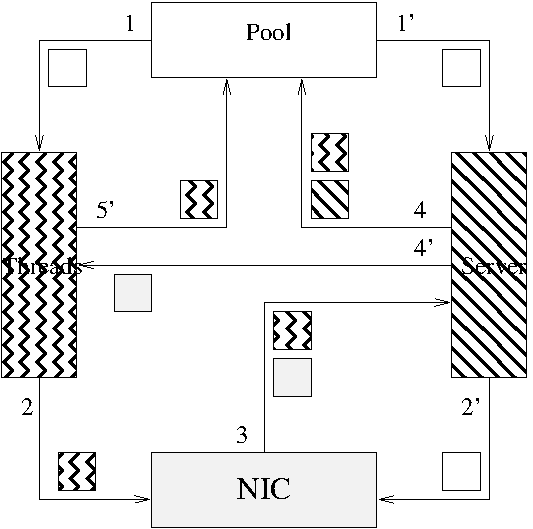
\includegraphics[width=0.3\textwidth]{fig/packetlife.pdf}
  \caption{Packet life cycle: (1) A thread sending data obtain a packet from the
    pool; (2) The thread writes data into the packet and submit it to the NIC;
    (1', 2') Communication server obtains a packet for receiving data
    and posts the packet to the NIC;
    (3) The server polls the NIC and obtains the packet back (either send/recv packet).
    (4) If the packet is for sending, it is returned to the pool;
    If the packet is for receiving and there is a request, the server copies the data
    and returns the packet to the pool;
    (4') If the packet is for receiving and the there is no request, the packet is inserted to hash-table.
    (5') The thread takes packet from the hash-table copies the data before returning it back to the pool.}
  
  \label{fig:packetlife}
\end{figure}

Figure \ref{fig:packetlife} explains how different components in our system
might change the affinity of data inside a packet. The figure shows the life of
a packet from the time it leaves the pool until it is returned. As explained in
the figure, when a packet returns to the pool, it can only has the affinity
of either the communication server or one of the worker thread. More specifically,
if the packet is used for sending data, it shall have the locality of the thread;
if the packet is used for receiving data, it shall have the locality of either
the thread or the server depending on whether the associated request and the
packet is received first. Moreover, when the packet is posted by the server
to the NIC for receiving data, the packet shall lose any affinity it has since
the NIC will perform a write over the packet.

Analysing the packet life cycle motivates us a new design for the packet pool.
We split the centralized packet management into a private pool per worker and a
shared pool per communication worker. Initially, there is a fixed number of
packets for each of the pool. At runtime, we design an algorithms to allow
moving packets among those pool depending on their usages.  Our goal is to
maintain good locality per hardware thread but does not block if there is
available resources.

The private pool consists of packets that are identified as having affinity of
the associated hardware thread. It is implemented as a fixed size double-ended
queue (deque). The deque has three main operations: \texttt{popTop},
\texttt{pushTop}, and \texttt{popBottom} which allows LIFO accessing at the top
of the queue, and also allows poping from its bottom. The idea is that at the
bottom of the deque are packets that are least recently used and are better
candidates for other purposes. That is, when the private pool is full, it
performs \texttt{popBottom} and pushed back to the shared pool.

When a packet for sending is needed by a thread, a \texttt{popTop} is performed
with the private pool of the current worker, which guarantees giving the last
packet that was read or written by the same worker. If the private pool is
empty, the shared pool is accessed for extra packets.  Alternatively, when a
packet is needed for receiving data by the communication server, the server
first try to obtains packets from its shared pool. If the shared pool is empty,
the server now performs a \textit{steal} by randomly chosing a private pool and
perform the \texttt{popBottom} operation.

The private pools can be thought as caches, and the shared pool can be thought
as the main memory. When ``the cache'' is full, it evicts the least recently
used to the ``main memory''. Our heuristic essentially performs
resource-balancing among the set of packets by moving it around pools with the
locality taken into account. Since the private pool is only shared between a
worker thread and the communication server, currently we implemented it using a
simple fixed-size buffer with a spinlock. The shared pool is accessed by more
than two threads, thus implemented using a lock-free stack.


\section{Experiment}
\label{sec:exp}
\pgfplotstableread{data/tableinsert.dat}\mytableinsert
\pgfplotstableread{data/tablefind.dat}\mytablefind
\pgfplotstableread{data/pool.dat}\mytablepool

\begin{figure*}[ht]
  \centering
  \begin{adjustbox}{width=.8\textwidth}
    \subfigure[Latency per successful \texttt{insert}.]{
      \centering
      \begin{tikzpicture}[scale=.8]
        \begin{axis}[xlabel=N Threads, ylabel=Latency (usec), ymin=0, scaled ticks=false, tick label style={/pgf/number format/fixed},
            boxplot/draw direction=y,
            ytick distance={0.1},
            ymax={0.6},
            cycle list={{red},{blue},{black}},
            legend pos={north west}
          ]
          % hack to make legend
          \addlegendimage{area legend,fill=red,draw=black}; \addlegendentry{arr};
          \addlegendimage{area legend,fill=blue,draw=black}; \addlegendentry{ch};
          \addlegendimage{area legend,fill=black,draw=black}; \addlegendentry{tbb};

          \pgfplotsinvokeforeach{0,...,23}{
            \addplot+[boxplot prepared from table={table=\mytableinsert,
              row=#1, lower whisker=lw, upper whisker=uw, lower quartile=lq, upper quartile=uq,
            median=med, draw position=nthreads}, boxplot prepared] coordinates {};
          }
        \end{axis}
      \end{tikzpicture}
    }

    \subfigure[Latency per fail \texttt{insert} followed by an \texttt{erase}.]{
      \centering
      \begin{tikzpicture}[scale=.8]
        \begin{axis}[xlabel=N Threads, ylabel=Latency (usec), ymin=0, scaled ticks=false, tick label style={/pgf/number format/fixed},
            boxplot/draw direction=y,
            ytick distance={0.1},
            ymax={0.6},
            cycle list={{red},{blue},{black}},
            legend pos={north west}
          ]
          % hack to make legend
          \addlegendimage{area legend,fill=red,draw=black}; \addlegendentry{arr};
          \addlegendimage{area legend,fill=blue,draw=black}; \addlegendentry{ch};
          \addlegendimage{area legend,fill=black,draw=black}; \addlegendentry{tbb};

          \pgfplotsinvokeforeach{0,...,23}{
            \addplot+[boxplot prepared from table={table=\mytablefind,
              row=#1, lower whisker=lw, upper whisker=uw, lower quartile=lq, upper quartile=uq,
            median=med, draw position=nthreads}, boxplot prepared] coordinates {};
          }
        \end{axis}
      \end{tikzpicture}
    }
  \end{adjustbox}

  \caption{Latency of our hash-table implementation (\textit{arr}) in comparison
  to libcuckoo (\textit{ch}) and tbb concurrent hash map (\textit{tbb}).  Each
  hash-table is created with the initial size of $2^{16}$, the number of
  insertion per thread is chosen so that there is enough room and no expansion is
  required. TBB is also compiled with \textit{tbb-malloc} to improve performance.
  Latency exceeds an 0.5 microsecond is not shown.\label{fig:hash-table}}

\end{figure*}

\subsection{Component overheads}
In this section we evaluate our implementation of each individual component.
Understanding them individually gives us an idea on the minimum cost of the overall
system. 
\subsubsection{Concurrent Hash-Table}
To evaluate the overhead due to hash-table operations, we measure the latency 
on hash-table operations in the two following scenarios when performing them
in a number of POSIX threads:

\begin{itemize}
  \item A thread performs \texttt{insert} when there is no item with the same key.
  \item A thread performs \texttt{insert} and there is already items in the hash-table, and it subsequently
    performs \texttt{erase}.
\end{itemize}

 The two scenarios represent the only two possible runtime execution of the
 hash-table in our algorithms, thus measuring the latency in both cases give us
 an idea on how it will add to the overhead of MPI procedure. To justify the
 benefit of customization, we also compare ourselves to two popular general
 purposes hash-tables: libcuckoo implementing cuckoo hashing (\textit{ch})
 \cite{chasing}, and TBB concurrent hashmap (\textit{tbb}) \cite{tbb}. The
 experiment is to create threads and have each performed a fixed number of
 insertion (and erase) with different key to collect the mean latency. We ran
 the experiment for $1000$ times and collect the summaries of the latency of a
 thread. Between each run, we also perform a cache invalidation.

Figure~\ref{fig:hash-table} shows the result of our experiment. In both cases,
both TBB concurrent hash map and libcuckoo shows inconsistent latency when
there is more concurrent threads, which is the result of conflicts. Since our
hash-table is optimized for these patterns, our latency is almost always as low
as 50 nanosecond. This latency is consitent with our expectation that our cost
for the hash-table is equivalent to 2 memory writes.

\subsubsection{Thread scheduler}
TODO

\subsubsection{Concurrent Packet Pool}
\begin{figure}[ht]
  \centering
  \begin{tikzpicture}[scale=.9]
    \begin{axis}[xlabel=N Threads, ylabel=Latency (usec), ymin=0, scaled ticks=false, tick label style={/pgf/number format/fixed},
        boxplot/draw direction=y,
            %ytick distance={0.1},
        ymax={1},
            %cycle list={{red,dashed},{blue,dashed},{black,dashed},{red},{blue},{black}},
        cycle list={{red},{blue},{black}},
        legend pos={north west}
      ]
          % hack to make legend
          %\addlegendimage{area legend,fill=red,draw=black,dashed}; \addlegendentry{numa-cp};
          %\addlegendimage{area legend,fill=blue,draw=black,dashed}; \addlegendentry{stack-cp};
          %\addlegendimage{area legend,fill=black,draw=black,dashed}; \addlegendentry{queue-cp};
      \addlegendimage{area legend,fill=red,draw=black}; \addlegendentry{numa};
      \addlegendimage{area legend,fill=blue,draw=black}; \addlegendentry{stack};
      \addlegendimage{area legend,fill=black,draw=black}; \addlegendentry{queue};

      \pgfplotsinvokeforeach{0,...,23}{
        \addplot+[boxplot prepared from table={table=\mytablepool,
          row=#1, lower whisker=lw, upper whisker=uw, lower quartile=lq, upper quartile=uq,
        median=med, draw position=nthreads}, boxplot prepared] coordinates {};
      }
    \end{axis}
  \end{tikzpicture}
  \caption{Latency of pool implementation vs. a lockfree pool and a lockfree queue
    implementation, latency higher than 1 microsecond are not shown\label{fig:pool}.}
  \end{figure}

The overhead due to packet pool is measured as the sum of the latency of
\texttt{get} and \texttt{ret} operation. We evaluate this quantity by
performing a random number of \texttt{get} followed by the same number of
\texttt{ret} in each thread. To match better with the real workload, we also
perform a random sleep in between the two group of operations. Further, The
range of the random number is chosen with the same seed for each implementation
and ensure threads do not request more than available packets: the maximum is
number of packets divided by number of threads. We perform this experiment
$1000$ times and plot the summary similarly as  the hash-table experiment.

The result is shown in Figure \ref{fig:pool} in comparison with implementation
using a concurrent lockfree stack and a lockfree queue. Our result for this
benchmark outperforms others by a wide margin, especially when the number of
threads increase. The lockfree stack is faster than the queue at single thread,
however performs worst for more than two threads since there is contention at
the top of the stack. The great variation in latency per operation of a
centralized pool is clearly due to memory conflicts in this type of access
patterns. Our latency is consistently in the range of 100-150 nanosecond.


\subsection{Microbenchmarks and Application Evaluation}
\begin{figure*}[ht]
  \centering
  \begin{adjustbox}{width=.9\textwidth}
    \subfigure[Latency per message transfer for $14$ threads, one per worker/socket.] {
      \centering
      \begin{tikzpicture}[scale=.9]
        \begin{axis}[xlabel=Message Size (byte), ylabel=Latency (usec),
            xmode=log, ymode=log, xtick distance=2^2,
            log basis x=2, log basis y=2,
            ymin=1, ytick distance=2^2,
            xmax=2^14,
            xmin=1, % cycle list={{red},{blue},{black}},
            legend pos={north west},
            mark size=1.5pt,
            legend style={font=\tiny},
            ylabel near ticks,
            xlabel near ticks,
          ]
          \addplot table [x=threads, y=mvapich2+mt] {data/pingpong2.dat} node[pos=0.27, pin=below:56.8]{};
          \addlegendentry{mvapich2+mt}
          \addplot table [x=threads, y=pthread+hash] {data/pingpong2.dat} node [pos=0.25, pin=above:5.7]{};
          \addlegendentry{pthread+hash}
          \addplot table [x=threads, y=abt+hash] {data/pingpong2.dat} node [pos=0.25, pin=above:2.3]{};
          \addlegendentry{abt+hash}
          \addplot table [x=threads, y=fult+hash] {data/pingpong2.dat} node [pos=0.25, pin=above:1.7]{};
          \addlegendentry{fult+hash}
        \end{axis}
      \end{tikzpicture}
    }
    \subfigure[Latency per 64-byte message transfer for upto 1M thread and round-robin assigned to worker/socket, 
      \textit{pthread+hash} version only works up to 16K threads due to limitation in the system.] {
      \centering
      \begin{tikzpicture}[scale=.9]
        \begin{axis}[xlabel=N threads, ylabel=Latency (usec),
            xmode=log, ymode=log, xtick distance=2^2,
            log basis x=2, log basis y=2,
            ymin=1, ytick distance=2^2,
            xmin=4,
            legend pos={north west},
            mark size=1.5pt,
            legend style={font=\tiny},
            yticklabel=\pgfmathparse{2^\tick}\pgfmathprintnumber{\pgfmathresult},
            ylabel near ticks,
            xlabel near ticks,
          ]
          \addplot table [x=threads, y=pthread+hash,col sep=comma] {data/strong.dat} node[pos=0.9, pin=7.9] {};
          \addlegendentry{pthread+hash}
          \addplot table [x=threads, y=abt+hash, col sep=comma] {data/strong.dat} node[pos=0.55, pin=2.3] {};
          \addlegendentry{abt+hash}
          \addplot table [x=threads, y=fult+hash, col sep=comma] {data/strong.dat} node[pos=0.55, pin=1.7] {};
          \addlegendentry{fult+hash}
        \end{axis}
      \end{tikzpicture}
    }
%    \subfigure[Number of worker = 14, Number of threads = 42] {
%      \begin{tikzpicture}[scale=.9]
%        \begin{axis}[xlabel=Message Size (byte), ylabel=Latency (usec),
%            xmode=log, ymode=log, xtick distance=2^2,
%            log basis x=2, log basis y=2,
%            ymin=1, ytick distance=2^2,
%            xmax=2^14,
%            xmin=1, % cycle list={{red},{blue},{black}},
%            legend pos={north west},
%            mark size=1.5pt,
%            legend style={font=\tiny},
%          ]
%          \addplot table [x=threads, y=mvapich2+mt] {data/pingpong3.dat};
%          \addlegendentry{mvapich2+mt}
%          \addplot table [x=threads, y=pthread+hash] {data/pingpong3.dat};
%          \addlegendentry{pthread+hash}
%          \addplot table [x=threads, y=abt+hash] {data/pingpong3.dat};
%          \addlegendentry{abt+hash}
%          \addplot table [x=threads, y=fult+hash] {data/pingpong3.dat};
%          \addlegendentry{fult+hash}
%        \end{axis}
%      \end{tikzpicture}
%    }
  \end{adjustbox}

  \caption{Latency comparison between different MPI implementation using OSU multi-threaded latency test.\label{fig:osumt}}
\end{figure*}

\subsubsection{OSU latency benchmarks}
\begin{table}
\begin{tabular}{|l|l|l|}
\hline
MPI impl. & Matching Algorithm & Scheduler \\
\hline
mvapich2+mt & queues & POSIX thread \\
\hline
pthread+hash & hash-table & POSIX thread \\
\hline
abt+hash & hash-table & Argobots \\
\hline
fult+hash & hash-table & Bitvector \\
\hline
\end{tabular}
\caption{Summary of MPI implementation used in the evaluation, Speedup is shown
  for latency test in Figure~\ref{fig:osumt} for message size of 64 bytes in
  comparison to mvapich2+mt.\label{tbl:mpi}}
\end{table}

We use OSU benchmarks \cite{osubench} to evaluate the latency per
\texttt{MPI_Send} or \texttt{MPI_Recv}. The single threaded test is performed
using \texttt{osu_latency}, the multi-threaded test is performed with
\texttt{osu_latency_mt}. We compare our best implementation
(\textit{fult+hash}) with MVAPICH2 and other possible implementation of our
runtime design.  Table~\ref{tbl:mpi} summarizes the differences of the tested
runtime.  \textit{mvapich2+mt} is the MVAPICH2 with POSIX thread which is the
base implementation in \texttt{osu_latency_mt}. Further, in multi-threaded test,
we modify the code so that each thread uses different tags.

Performance results for multi-threaded tests are shown in
Figure~\ref{fig:osumt}.  Under tested settings, the most improvement in
performance is due to the replacement of the complex queue of MPI with the
hash-table.  Then, the replacement of POSIX threads with a light-weight
threads. Our thread-scheduler improves the latency upto 40\% compared to
Argobots, $3$ times compared to POSIX thread scheduler. Overally, we achieve
speedup of upto $45\times$ compared to MVAPICH2.

\begin{figure}
  \centering
  \begin{tikzpicture}[scale=0.9]
    \begin{axis}[xlabel=Message Size (byte), ylabel=Latency (usec),
        xmode=log, ymode=log, xtick distance=2^2,
        log basis x=2, log basis y=2,
        xmax=2^14,
        xmin=1, % cycle list={{red},{blue},{black}},
        legend pos={north west},
        mark size=1.5pt,
        legend style={font=\tiny},
      ]
      \addplot table [x=threads, y=mvapich2+mt] {data/pingpong1.dat} node[pos=0.24, pin=above:1.7]{};
      \addlegendentry{mvapich2+mt}
      \addplot table [x=threads, y=pthread+hash] {data/pingpong1.dat};
      \addlegendentry{pthread+hash}
      \addplot table [x=threads, y=abt+hash] {data/pingpong1.dat} node[pos=0.24, pin=above:1.85]{};
      \addlegendentry{abt+hash}
      \addplot table [x=threads, y=fult+hash] {data/pingpong1.dat} node[pos=0.24, pin=right:1.45]{};
      \addlegendentry{fult+hash}
      \addplot table [x=threads, y=mvapich2] {data/pingpong1.dat} node[pos=0.24, pin=right:1.23]{};
      \addlegendentry{mvapich2}
    \end{axis}
  \end{tikzpicture}
  \caption{Latency comparison for single-threaded OSU latency test.\label{fig:osu-single}}
\end{figure}

Our overheads analyzed in the previous section translate accurately to the
single-threaded benchmark results in Figure~\ref{fig:osu-single}. In general,
compared to a single-threaded MPI implementation, our best implementation
achieves overall overhead of 0.2 $usec$ virtually tie with running MPI
in a POSIX thread in MPI_THREAD_MULTIPLE mode (as in \textit{mvapich2+mt}).


\section{Related Works}
\label{sec:related}

\section{Conclusion}
\label{sec:conclusion}

\bibliographystyle{abbrv}
\bibliography{mpiv}
\end{document}
